% Owner: Sharjeel Shahid 24L-3055
\section{Application (Track A)}
\label{sec:application}

\subsection{Why Track A and Streamlit}
Track A is implemented as a local web application that connects the saved
models to a supplier-quote decision. Streamlit~\cite{b_streamlit} keeps the
interface in Python, the same language as preprocessing and inference, and
provides interactive controls without a separate front-end implementation.
Once dependencies and saved artifacts are present, the application starts
with one command. A hosted service is not required for this demonstration.
Here ``real-time inference'' means computing a result when the user requests
it; it does not mean a streaming market feed or a measured latency guarantee.
Response time and concurrent-user capacity were not measured for this report.

\subsection{Application Architecture}
The entry point, \texttt{app/streamlit\_app.py}, registers four pages using
\texttt{st.Page} and top navigation: Quote Check, Market, Model Insights and
About. The page scripts call inference and recommendation functions, which
read the saved models and data. This is the application-facing part of the
pipeline in Figure~\ref{fig:system}; the architecture image is not repeated
here.

\begin{itemize}
    \item \textbf{Quote Check} --- \texttt{app/views/quote\_check.py}: reads
    cleaned prices, feature metadata, the saved scaler, classical model
    bundles, the LSTM checkpoint/configuration and the test comparison table.
    User uploads and downloaded prices provide alternative in-memory inputs.
    \item \textbf{Market} --- \texttt{app/views/market.py}: reads
    \texttt{data/processed/cleaned.csv} through
    \texttt{src.\allowbreak inference.\allowbreak features.\allowbreak load\_\allowbreak builtin\_\allowbreak prices()}.
    \item \textbf{Model Insights} --- \texttt{app/views/model\_insights.py}:
    reads saved prediction, comparison, tuning, history and bias/segment CSVs
    under \texttt{results/}, together with existing report figures.
    \item \textbf{About} --- \texttt{app/views/about.py}: reads dataset dates,
    the training feature header, model comparison and bias tables,
    \texttt{README.md} for the team, and the saved pipeline figure.
\end{itemize}

The inference and recommendation entry points are:
\begin{itemize}
    \item \texttt{src.\allowbreak inference.\allowbreak features}:
    \texttt{build\_\allowbreak features()}.
    \item \texttt{src.\allowbreak inference.\allowbreak classical}:
    \texttt{predict\_\allowbreak classical()}.
    \item \texttt{src.\allowbreak inference.\allowbreak lstm}:
    \texttt{predict\_\allowbreak lstm()}.
    \item \texttt{src.\allowbreak inference.\allowbreak live}:
    \texttt{download\_\allowbreak latest()}.
    \item \texttt{src.\allowbreak recommendation.\allowbreak price\_\allowbreak range}:
    \texttt{check\_\allowbreak quote()} calls \texttt{expected\_\allowbreak range()}
    and \texttt{recommend()} to produce the action and its explanation.
\end{itemize}

The pages reuse Deliverable 1 transformations and Deliverable 2 weights; they
do not train models or regenerate evaluation artifacts. Application access
to \texttt{data/}, \texttt{models/}, \texttt{results/} and
\texttt{report/figures/} is read-only. This is an artifact-preservation
statement, not a claim that the whole process cannot write: reused collection
and cleaning helpers contain file-logging setup and logging calls.

\subsection{Real-Time Inference Flow}
% Sources: quote_check.py; features.py; classical.py; lstm.py; lstm_config.json; price_range.py.
The user chooses the metal, data source, quoted price and quantity, then
presses \textbf{Check quote}. For gold, logistic regression is the default
model because it is the first entry in \texttt{MODEL\_NAMES}. The other
classical options are random forest and gradient boosting; the majority
baseline is a results-page comparator, not a quote-check model option.

The cached \texttt{gold\_probabilities()} helper calls
\texttt{build\_features()} on the chosen prices. This reuses
\texttt{data\_scripts.feature\_engineering.build\_features()}, the training
return caps derived from \texttt{features\_unscaled.csv}, and
\texttt{data/processed/scaler.joblib}. The result follows the 27-column
training feature schema, excluding the future-price and direction targets.
The saved scaler transforms its designated numeric columns; binary and
calendar features retain their prescribed representation. Temporary repeated
price rows allow feature construction at the latest observed date; the
future targets and the padding rows are then removed, rather than supplied
as model inputs.

\texttt{predict\_classical()} selects each saved bundle's feature columns
from the final row and returns its \texttt{predict\_proba} up-probability.
\texttt{predict\_lstm()} uses the saved configuration: a 60-trading-day
window and 14 stationary features selected from the same frame. CPU inference
runs with evaluation mode and gradients disabled, followed by a sigmoid.
Classical models are cached by \texttt{load\_model()} using
\texttt{lru\_cache}; the LSTM model and configuration have a module-level
cache. Streamlit also caches data and computed probabilities in memory.

An LSTM probability is displayed only after PyTorch, the configuration and
weights load successfully. Missing dependencies, weights or invalid input
cause the probability to be omitted. There is a narrower interface
limitation: because PyTorch is imported lazily, the LSTM selector option can
remain visible even when its weights or PyTorch are unavailable. Selecting
it then leaves no LSTM probability, so the recommendation uses the price
range alone. The selector itself is not a complete availability check.

For gold, \texttt{check\_quote()} combines the selected probability with a
five-trading-day price range. \texttt{expected\_range()} applies the 10th,
50th and 90th percentiles of historical five-day returns through
31 December 2021 to the latest price. A quote above the upper bound leads to
\textbf{Negotiate}; one below the lower bound leads to \textbf{Buy}. Within
the range, an up-probability of at least 50\% leads to \textbf{Buy}, otherwise
\textbf{Hold}. Without a model probability, the median range value replaces
the probability decision. The displayed result includes reasons, the market
price, quote difference and cost comparison for the entered quantity.
Silver, copper and platinum always use the historical range only.

\subsection{Data Options on Quote Check}
% Sources: cleaned.csv date extrema; quote_check.py; features.py; live.py.
\begin{itemize}
    \item \textbf{Built-in data.} \texttt{load\_builtin\_prices()} loads the
    frozen cleaned table. The inspected dataset runs from 4 January 2010 to
    21 October 2026; the page derives its displayed dates from the file rather
    than treating them as today's prices.
    \item \textbf{Upload CSV.} Required columns are \texttt{date},
    \texttt{gold}, \texttt{silver}, \texttt{copper}, \texttt{platinum},
    \texttt{dxy}, \texttt{wti}, \texttt{us10y} and \texttt{cpi}.
    \texttt{read\_upload()} checks column names and dates, sorts the rows,
    removes weekends and duplicates, and reuses the cleaning functions for
    missing values, impossible prices and outlier flags. At least 100
    trading-day rows must remain after cleaning. Parsing, missing-column,
    date and insufficient-history errors are shown as messages. A downloadable
    template is built from the final 120 rows of the built-in prices.
    \item \textbf{Latest prices.} \texttt{download\_latest(days=365)} requests
    about one year of prices. Metals, the dollar index, oil and the yield
    backup come from Yahoo Finance; CPI comes from the US Bureau of Labor
    Statistics. It forward-fills CPI, excludes the current day and applies
    the upload-cleaning path. Internet access is required, and download
    failures produce an error message. Returned prices are passed through
    an in-memory \texttt{StringIO} CSV, not saved as a dataset. The page caches
    this result for 3,600 seconds. The logging qualification above still
    applies, so ``nothing is saved to disk'' would be too broad a claim.
\end{itemize}

The current implementation loads built-in data before enabling the other
sources, and uses its earlier prices as historical context for range
estimation. Upload and Latest prices therefore do not remove the need for
the local reference dataset. If classical weights are missing, the page
reports that AI inference could not run and falls back to the price range
for the handled error cases.

\subsection{Screenshots}
The following figure slots correspond to the four application pages.
Their descriptions are verified against the page code and saved data.
Where a screenshot file is unavailable, the slot explicitly states this;
dataset dates are not asserted to be screenshot capture dates.

\paragraph{Quote Check.}
The page accepts the supplier quote and quantity, explains the recommendation,
and displays the selected model's role alongside the expected price range.
\begin{figure}[H]
    \centering
    \IfFileExists{figures/app/quote_check.png}{%
        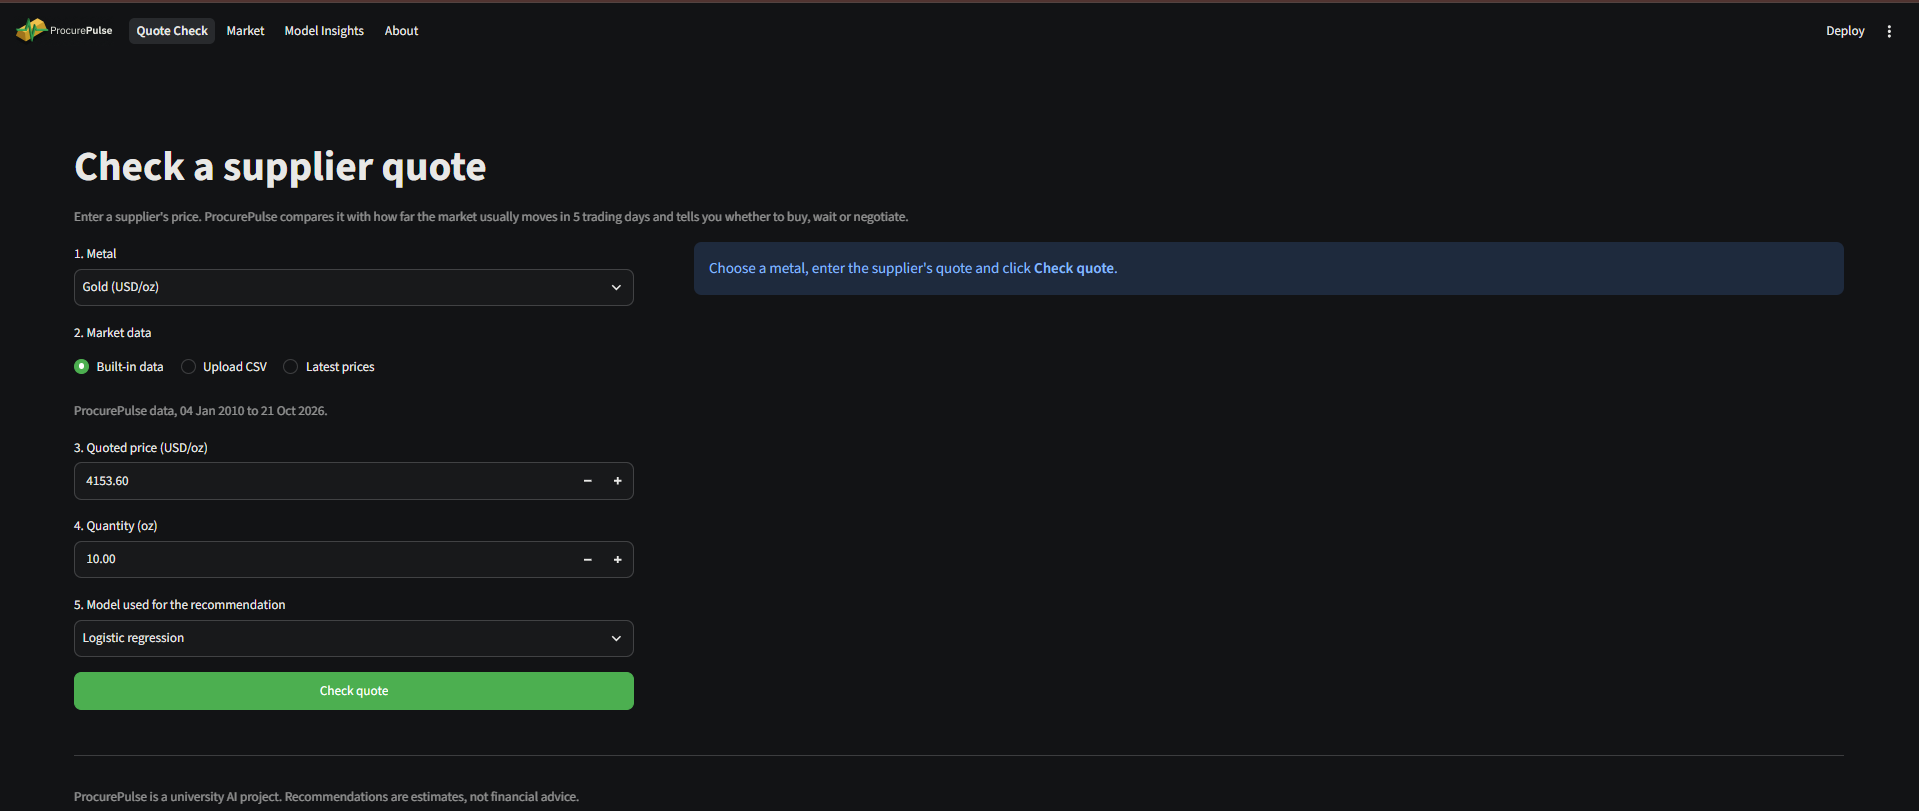
\includegraphics[width=0.9\textwidth,height=0.85\textheight,keepaspectratio]{app/quote_check.png}%
    }{\fbox{\parbox{0.85\textwidth}{Quote Check screenshot is not available.}}}
    \caption{Quote Check: data-source and quote controls, recommendation and price-range explanation. The inspected built-in data ends on 21 October 2026.}
    \label{fig:b-app-quote-check}
\end{figure}

\paragraph{Market.}
The page offers eight series, a date-range filter, prices with a 30-day
average or daily returns, and summaries of price change, volatility and
outlier days. An outlier flag belongs to the day, not to an individual
series. Gold--dollar and gold--oil comparisons rescale each series over the
selected interval.
\begin{figure}[H]
    \centering
    \IfFileExists{figures/app/market.png}{%
        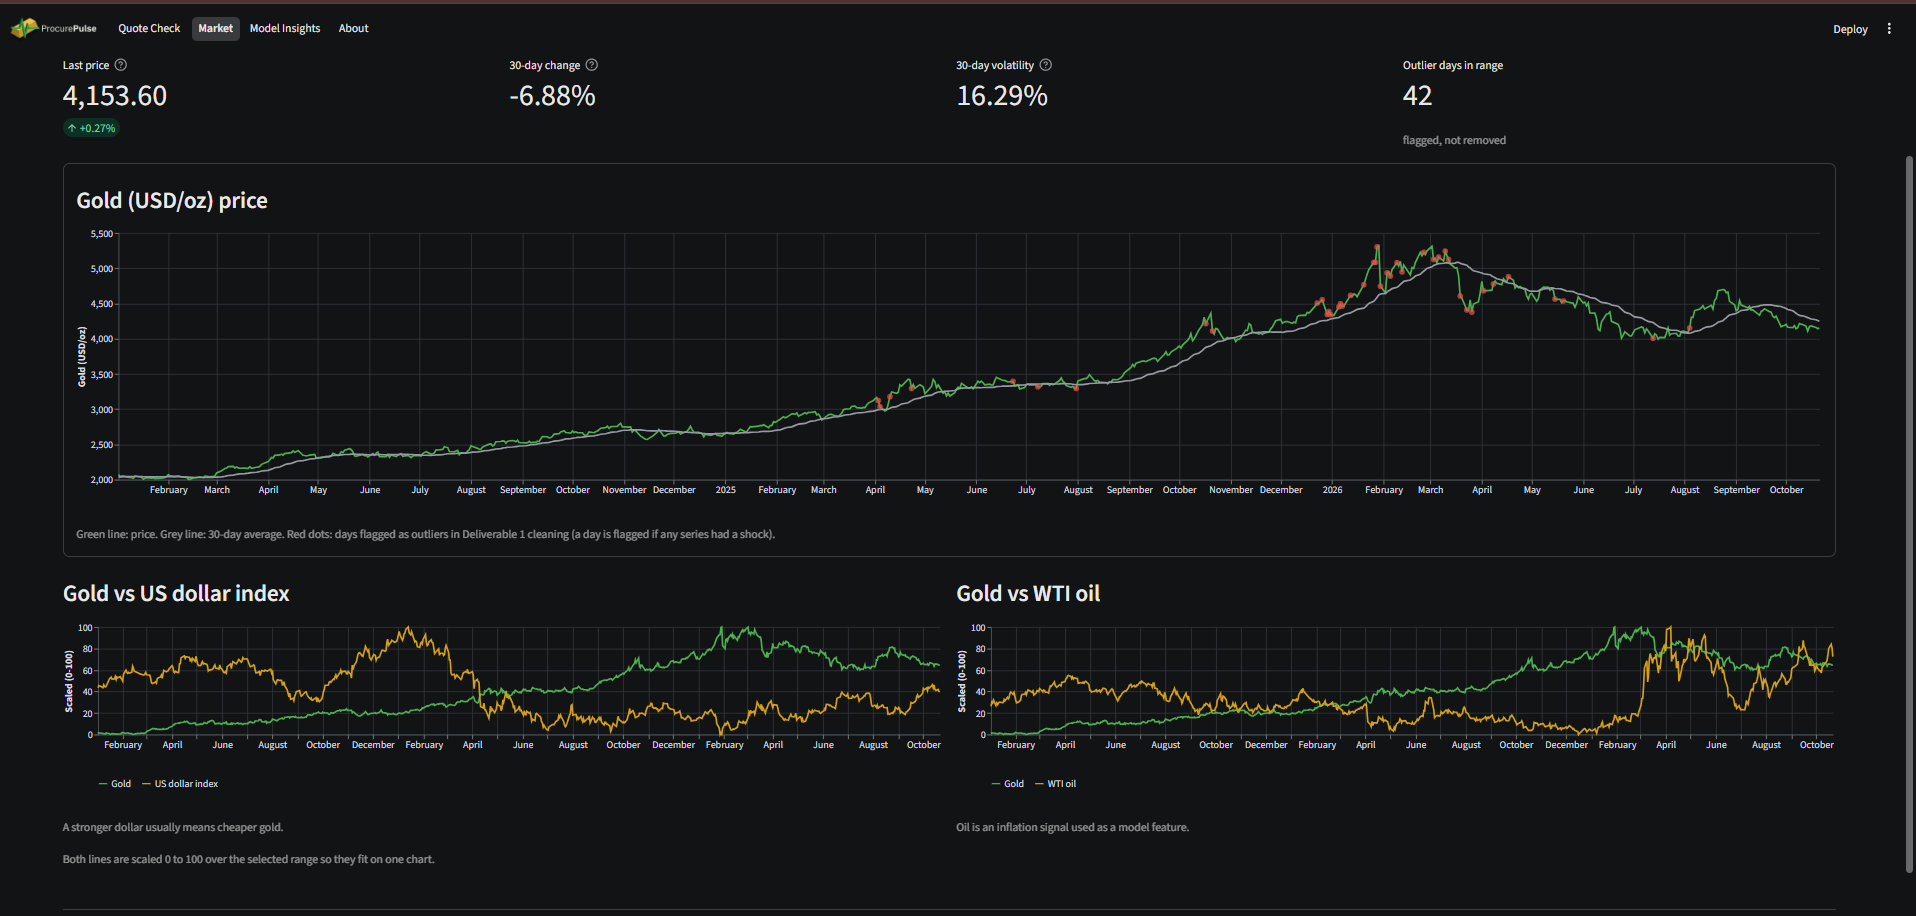
\includegraphics[width=0.9\textwidth,height=0.85\textheight,keepaspectratio]{app/market.png}%
    }{\fbox{\parbox{0.85\textwidth}{Market screenshot is not available.}}}
    \caption{Market: historical series controls, trend and outlier views, and gold comparisons. The inspected dataset covers 4 January 2010--21 October 2026.}
    \label{fig:b-app-market}
\end{figure}

\paragraph{Model Insights.}
Its Overview, Training, Errors and Bias, and Sample predictions tabs expose
saved metrics, learning curves, tuning tables, prediction imbalance and
recent test probabilities. These are existing evaluation results, not
recomputed model scores from the quote the user enters.
\begin{figure}[H]
    \centering
    \IfFileExists{figures/app/model_insights.png}{%
        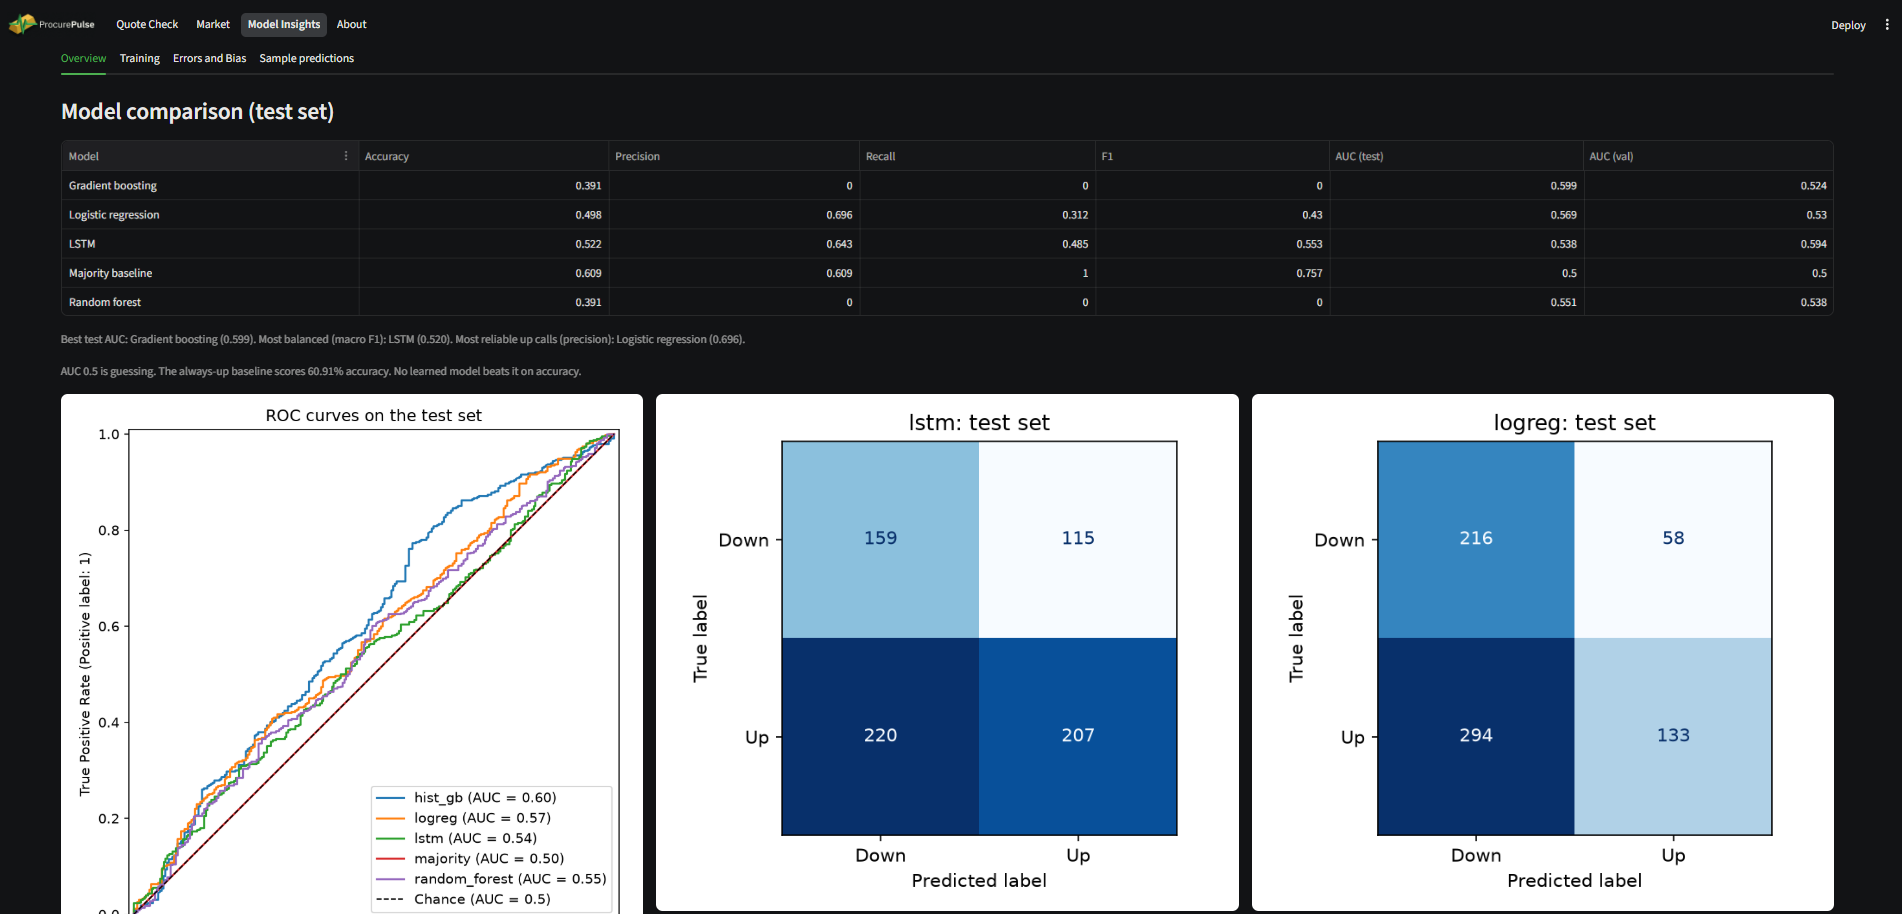
\includegraphics[width=0.9\textwidth,height=0.85\textheight,keepaspectratio]{app/model_insights.png}%
    }{\fbox{\parbox{0.85\textwidth}{Model Insights screenshot is not available.}}}
    \caption{Model Insights: comparison and diagnostic views of the saved results. The prediction files contain 701 test days from 2 January 2024 to 14 October 2026.}
    \label{fig:b-app-model-insights}
\end{figure}

\paragraph{About.}
The page describes the project, data options, limitations and team, with
Terms of Service and Privacy Policy expanders. Data dates, feature count and
best test AUC are derived from saved files; team information comes from the
README. Missing supporting files produce availability messages.
\begin{figure}[H]
    \centering
    \IfFileExists{figures/app/about.png}{%
        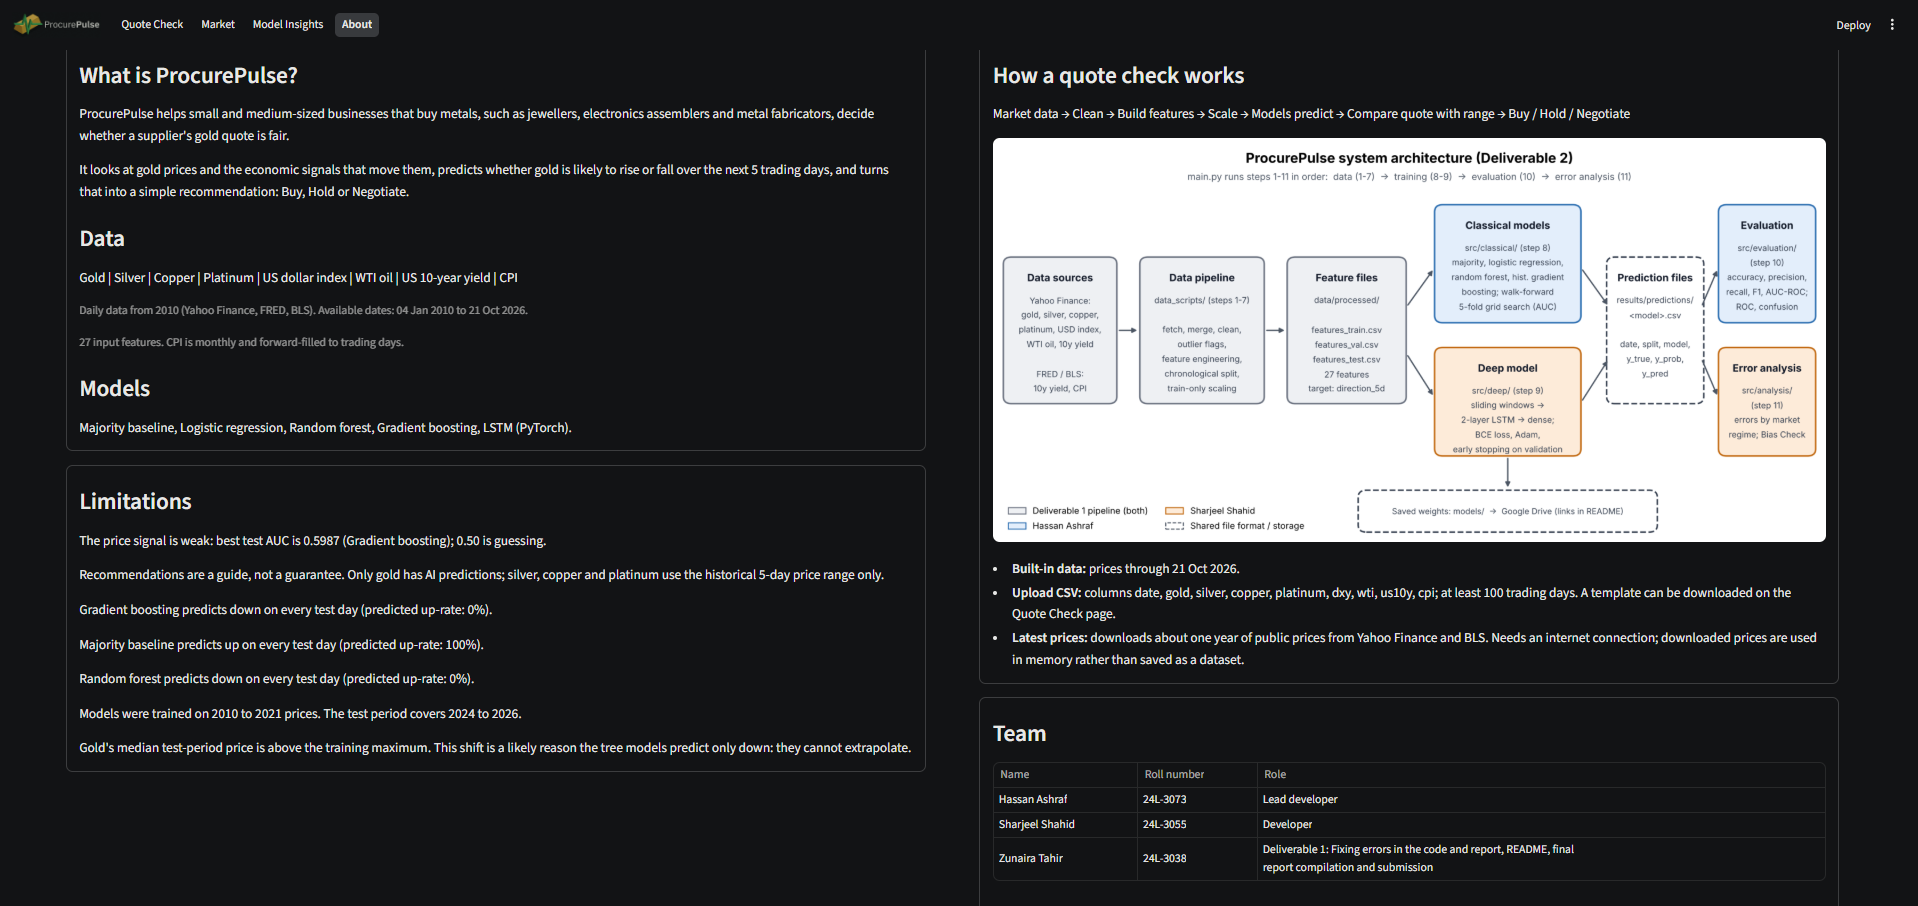
\includegraphics[width=0.9\textwidth,height=0.85\textheight,keepaspectratio]{app/about.png}%
    }{\fbox{\parbox{0.85\textwidth}{About screenshot is not available.}}}
    \caption{About: project context, data choices, limitations, team and policies. Its inspected built-in-data endpoint is 21 October 2026.}
    \label{fig:b-app-about}
\end{figure}

\subsection{Sample Predictions}
% Sources: logreg.csv and lstm.csv, split=test, sorted by date, tail(120).
Figure~\ref{fig:b-app-sample-predictions} uses the last 120 test dates in each
saved prediction file, 24 April--14 October 2026. The line is the predicted
probability that gold rises over the next five trading days; the green and
red dots show the realised binary outcomes. Classification uses
$\hat y=\mathbf{1}[p\geq 0.5]$.

\begin{figure}[H]
    \centering
    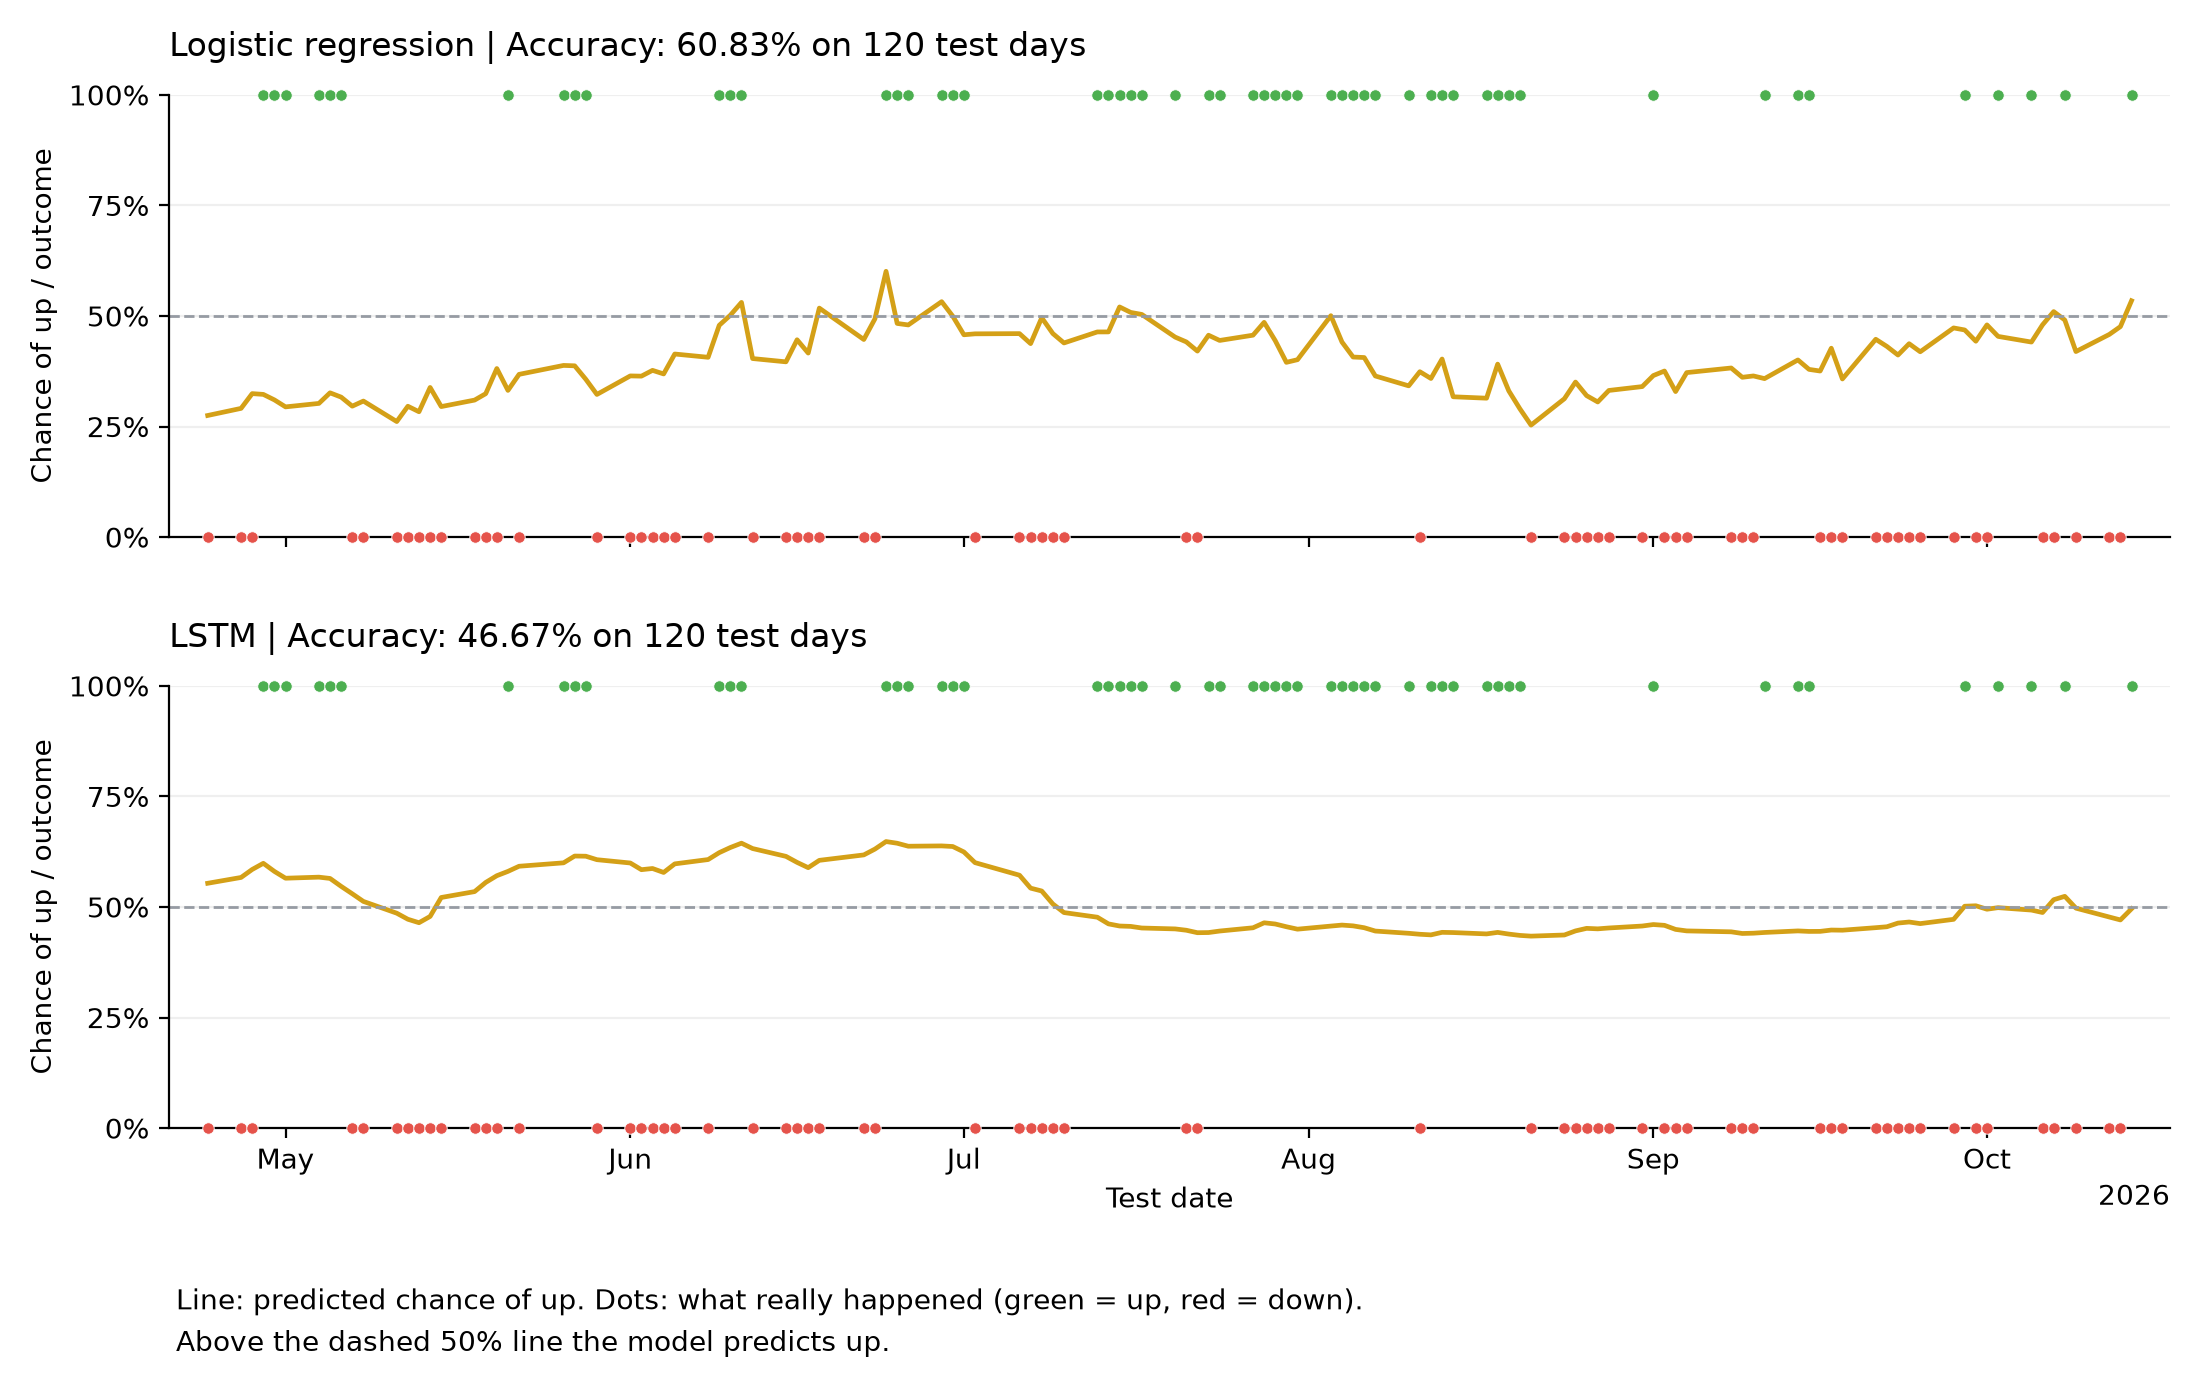
\includegraphics[width=\textwidth]{analysis/sample_predictions.png}
    \caption{Saved logistic-regression and LSTM probabilities on the final 120 test days, 24 April--14 October 2026. Green dots denote actual up outcomes and red dots down or flat outcomes; the dashed line is the 50\% decision threshold.}
    \label{fig:b-app-sample-predictions}
\end{figure}

Logistic regression classifies 73 of these 120 outcomes correctly
(60.83\% accuracy), while the LSTM classifies 56 correctly (46.67\%).
Logistic regression is below 50\% on 109 dates and above it on 11; the LSTM
is below on 68 dates and above on 52. Neither has an exact threshold tie.
Both therefore favour down predictions in this interval, especially logistic
regression. These percentages are rounded to two decimal places, matching
the figure.

The full-test AUC values in \texttt{model\_comparison.csv} are 0.5690 for
logistic regression and 0.5377 for the LSTM. They indicate weak discrimination
above the 0.5 chance reference, not dependable trading signals. This recent
window is a visual check of saved outputs, not an independent new test or
evidence of profitability. Transaction costs and purchasing profit were not
measured by this figure.

\subsection{Running the Application and Limitations}
From the repository root, with the project environment active, run:
\begin{verbatim}
python -m streamlit run app/streamlit_app.py
\end{verbatim}
Install the dependencies in \texttt{requirements.\allowbreak txt}, which
specifies \texttt{streamlit>=1.46}. The inspected environment has Streamlit
1.67.0. Follow the README's artifact layout. Keep classical \texttt{.joblib}
bundles in \texttt{models/\allowbreak classical/}, and
\texttt{lstm\_\allowbreak best.\allowbreak pt} with
\texttt{lstm\_\allowbreak config.\allowbreak json} in
\texttt{models/\allowbreak deep/}. Keep the cleaned prices, feature CSVs,
unscaled features and \texttt{scaler.\allowbreak joblib} under
\texttt{data/\allowbreak processed/}. Retain saved results and figures for
the diagnostic pages. Starting this interface does not require rerunning
the README's training pipeline.

The predictive signal remains weak. In \texttt{bias\_check.csv}, random
forest and gradient boosting have a test predicted up-rate of zero: both
predict down throughout the saved test period. The price-level distribution
shift discussed in Section~\ref{sec:error-bias} is a plausible explanation,
not a causal effect established by this interface. AI predictions are
available only for gold; Latest prices depends on internet access and
external providers. This is a local demonstration, not a hosted production
service, and its recommendations are estimates rather than financial advice.
